\subsection{Mockup}
Pada perancangan antar muka sistem akan dibuat tampilan untuk aplikasi presensi \textit{online} berupa \textit{website}. Pada perancangan tampilan ini akan dibuat \textit{mockup} untuk merepresentasikan tampilan antar muka dari aplikasi. Menurut Uzayr~\cite{mastering2022sufyan}, \textit{mockup} adalah model visual dari antarmuka pengguna (UI). \textit{Mockup} memudahkan desainer untuk fokus pada visual produk. \textit{Mockup} membantu pengguna atau pemangku kepentingan untuk memahami bentuk akhir produk pada tahap awal. Saat ini, alat \textit{mockup} semakin mendapat perhatian karena membantu membangun spesifikasi UI dengan melibatkan pengguna.

\subsection{Windows Navigation Diagram}
\textit{Windows navigation diagram} akan menguraikan semua menu dalam aplikasi presensi \textit{online}. Diagram ini menyediakan peta visual yang membantu pengguna memahami struktur dan alur aplikasi presensi \textit{online}.

\subsubsection{Antar Muka Aplikasi Presensi \textit{Online}}
Aplikasi presensi \textit{online} terdapat menu \textit{login} sebagai menu pertama yang akan tampil ketika pengguna membuka url utama dari \textit{website} dan akan mengecek \textit{credential} pada pengguna. Jika sebelumnya pengguna sudah login maka akan langsung mengalihkan halaman ke menu utama. Jika tidak ada \textit{credential} maka halaman akan tetap pada menu \textit{login}. Seluruh menu dan jalur akses dari setiap menu pada aplikasi presensi \textit{online} dapat dilihat pada \textbf{\ref{fig:windows-navigation-diagram-aplikasi-presensi-online}}.
%
\begin{figure}[!htbp]
	\centering
	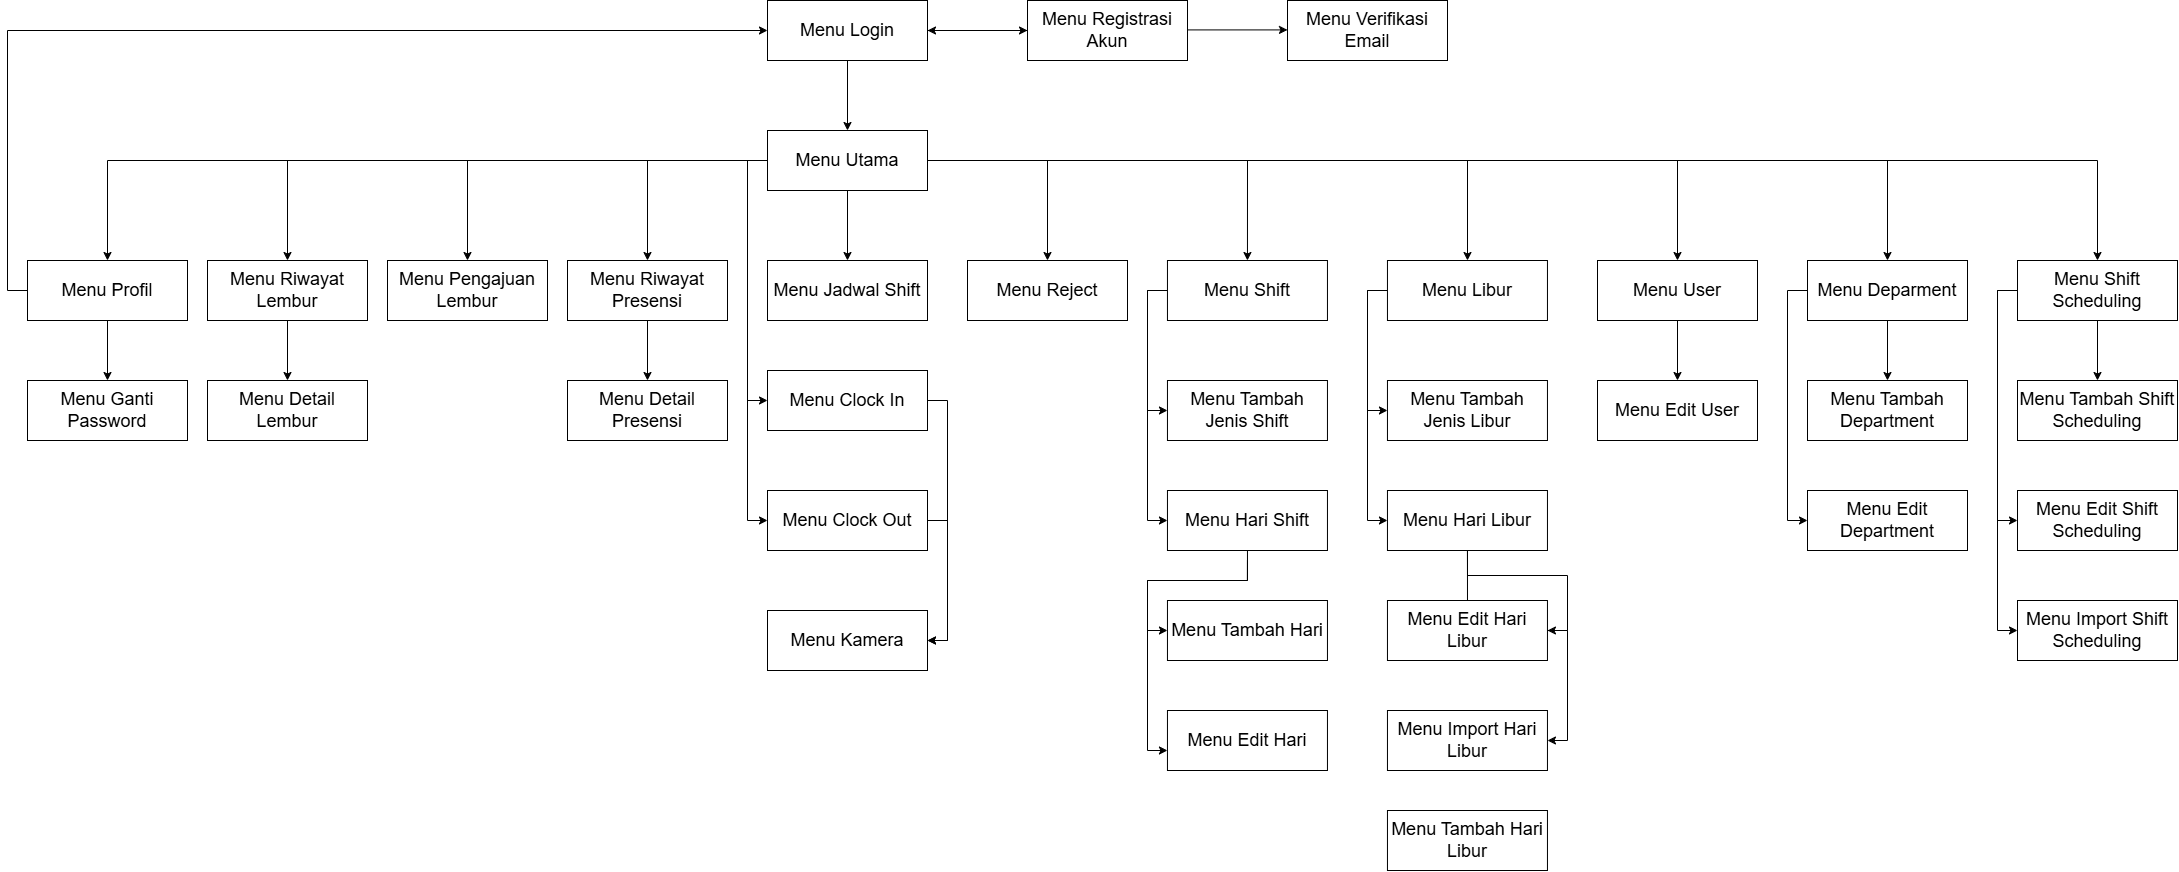
\includegraphics[width=15cm]{Gambar/bab2/windows-navigation-diagram.png}
	\caption{\textit{Windows Navigation Diagram} Aplikasi Presensi \textit{Online}}
	\label{fig:windows-navigation-diagram-aplikasi-presensi-online}
\end{figure}
\FloatBarrier

Pada aplikasi presensi \textit{online} terdiri dari 36 menu yaitu.
\begin{enumerate}
    \item Menu \textit{Utama}
    \\ Menu Utama adalah menu pertama yang muncul saat pengguna membuka aplikasi melalui tautan URL di \textit{website}. Halaman ini hanya dapat diakses ketika pengguna sudah \textit{login} sebelumnya, jika pengguna belum \textit{login} maka akan mengalihkan halaman ke Menu \textit{Login}. Menu ini juga digunakan oleh \textit{staff Infrastructure} untuk melakukan presensi. Tampilan Menu Utama dapat dilihat pada \textbf{\hyperref[sec:mockup-aplikasi-presensi-online]{Lampiran~XI}, \ref{fig:mockup-menu-utama}}.
    
    \item Menu \textit{Login}
    \\ Menu \textit{Login} merupakan menu yang berisi \textit{input form} untuk \textit{login} seluruh pengguna. Jika pengguna sudah \textit{login} sebelumnya maka halaman akan langsung dialihkan ke Menu Utama. Tampilan \textit{mockup} Menu \textit{Login} dapat dilihat pada \textbf{\hyperref[sec:mockup-aplikasi-presensi-online]{Lampiran~XI}, \ref{fig:mockup-menu-login}}.

    \item Menu Registrasi Akun
    \\ Menu Registrasi Akun merupakan halaman yang berisi \textit{input form} yang dapat digunakan oleh pengguna untuk membuat akun baru. Setelah pengguna mendaftar maka tinggal menunggu pengaktifan akun oleh \textit{manager}. Tampilan \textit{mockup} Menu Registrasi Akun dapat dilihat pada \textbf{\hyperref[sec:mockup-aplikasi-presensi-online]{Lampiran~XI}, \ref{fig:mockup-menu-registrasi-akun}}.

    \item Menu Verifikasi \textit{Email}
    \\ Menu Verifikasi \textit{Email} merupakan halaman menu yang menampilkan \textit{input form} kode OTP agar pengguna dapat melakukan verifikasi \textit{email} yang dikirimkan sistem setelah registrasi akun. Tampilan \textit{mockup} Menu Verifikasi \textit{Email} dapat dilihat pada \textbf{\hyperref[sec:mockup-aplikasi-presensi-online]{Lampiran~XI}, \ref{fig:mockup-menu-verifikasi-email}}.

    \item Menu Ganti Password
    \\ Menu Ganti Password merupakan halaman yang berisi \textit{input form} yang dapat digunakan oleh semua pengguna untuk membuat password baru akun. Tampilan \textit{mockup} Menu Ganti Password dapat dilihat pada \textbf{\hyperref[sec:mockup-aplikasi-presensi-online]{Lampiran~XI}, \ref{fig:mockup-menu-ganti-password}}.

    \item Menu Jadwal \textit{Shift}
    \\ Menu Jadwal \textit{Shift} merupakan halaman yang digunakan oleh \textit{staff Infrastructure} untuk melihat \textit{list} jadwal hari dan waktu \textit{shift} kerja. Tampilan \textit{mockup} Menu Jadwal \textit{Shift} dapat dilihat pada \textbf{\hyperref[sec:mockup-aplikasi-presensi-online]{Lampiran~XI}, \ref{fig:mockup-menu-jadwal-shift}}.

    \item Menu \textit{Clock In}
    \\ Menu \textit{Clock In} adalah halaman menu yang digunakan oleh \textit{staff Infrastructure} untuk melakukan presensi masuk. Menu ini dapat diakses ketika \textit{staff Infrastructure} menekan tombol \textit{clock in} pada Menu Utama. Pada menu ini terdapat tombol yang digunakan untuk mengambil lokasi dan tombol untuk menampilkan Menu Kamera. Tampilan \textit{mockup} Menu \textit{Clock In} dapat dilihat pada \textbf{\hyperref[sec:mockup-aplikasi-presensi-online]{Lampiran~XI}, \ref{fig:mockup-menu-clock-in}}.

    \item Menu \textit{Clock Out}
    \\ Menu \textit{Clock Out} adalah halaman menu yang digunakan oleh \textit{staff Infrastructure} untuk melakukan presensi keluar. Pada menu ini terdapat tombol untuk mengambil lokasi dan tombol untuk menampilkan Menu Kamera. Pada saat \textit{staff Infrastructure} melakukan \textit{clock out}, sistem akan mengecek data presensi saat \textit{clock in} dan \textit{clock out}, kemudian secara otomatis membuat data lembur jika presensi dilakukan diluar jam \textit{shift} atau pada hari libur. Tampilan \textit{mockup} Menu \textit{Clock Out} dapat dilihat pada \textbf{\hyperref[sec:mockup-aplikasi-presensi-online]{Lampiran~XI}, \ref{fig:mockup-menu-clock-out}}.

    \item Menu Kamera
    \\ Menu Kamera adalah menu yang digunakan oleh \textit{staff Infrastructure} untuk melakukan pengambilan foto wajah saat melakukan presensi masuk ataupun keluar. Tampilan \textit{mockup} Menu Kamera dapat dilihat pada \textbf{\hyperref[sec:mockup-aplikasi-presensi-online]{Lampiran~XI}, \ref{fig:mockup-menu-kamera}}.

    \item Menu Profil
    \\ Menu Profil adalah menu yang dapat digunakan oleh semua pengguna untuk melakukan \textit{logout} pada aplikasi dan menampilkan menu ganti password. Tampilan \textit{mockup} Menu Profil dapat dilihat pada \textbf{\hyperref[sec:mockup-aplikasi-presensi-online]{Lampiran~XI}, \ref{fig:mockup-menu-profil}}.

    \item Menu Pengajuan Lembur
    \\ Menu Pengajuan Lembur merupakan menu yang digunakan oleh \textit{staff Infrastructure} untuk membuat \textit{form} baru terkait lembur, jika \textit{staff} tersebut lupa melakukan presensi saat lembur. Tampilan \textit{mockup} Menu Pengajuan Lembur dapat dilihat pada \textbf{\hyperref[sec:mockup-aplikasi-presensi-online]{Lampiran~XI}, \ref{fig:mockup-menu-pengajuan-lembur}}.

    \item Menu Riwayat Presensi
    \\ Menu Riwayat Presensi dapat diakses oleh semua pengguna. Menu ini akan menampilkan \textit{list} data presensi yang telah dilakukan dan pengguna dapat melakukan \textit{filter} data agar dapat mencari data secara spesifik. \textit{Manager} dapat melihat seluruh presensi \textit{staff} dan melakukan \textit{export} data presensi dalam bentuk \textit{Microsoft Excel}, sedangkan \textit{staff} hanya dapat melihat presensi miliknya sendiri. Tampilan \textit{mockup} Menu Riwayat Presensi dapat dilihat pada \textbf{\hyperref[sec:mockup-aplikasi-presensi-online]{Lampiran~XI}, \ref{fig:mockup-menu-riwayat-presensi}}.

    \item Menu Detail Presensi
    \\ Menu Detail Presensi dapat diakses dengan memilih salah satu \textit{list} data presensi pada Menu Riwayat Presensi. Menu Detail Presensi menampilkan informasi lengkap dari suatu data presensi. Tampilan \textit{mockup} Menu Detail Presensi dapat dilihat pada \textbf{\hyperref[sec:mockup-aplikasi-presensi-online]{Lampiran~XI}, \ref{fig:mockup-menu-detail-presensi}}.

    \item Menu Riwayat Lembur
    \\ Menu Riwayat Lembur dapat diakses oleh semua pengguna. Menu ini akan menampilkan semua \textit{list} data lembur dan pengguna dapat melakukan \textit{filter} pada data lembur untuk mencari data yang lebih spesifik. \textit{Manager} dapat melihat semua data lembur dan melakukan \textit{export} data presensi dalam bentuk \textit{Microsoft Excel}, sedangkan \textit{staff} hanya dapat melihat data lembur miliknya sendiri. Tampilan \textit{mockup} Menu Riwayat Lembur dapat dilihat pada \textbf{\hyperref[sec:mockup-aplikasi-presensi-online]{Lampiran~XI}, \ref{fig:mockup-menu-riwayat-lembur}}.

    \item Menu Detail Lembur
    \\ Menu Detail Lembur dapat diakses dengan memilih salah satu \textit{list} data lembur pada Menu Riwayat Lembur. Menu Detail Lembur menampilkan informasi lengkap dari suatu data lembur. Tampilan \textit{mockup} Menu Detail Lembur dapat dilihat pada \textbf{\hyperref[sec:mockup-aplikasi-presensi-online]{Lampiran~XI}, \ref{fig:mockup-menu-detail-lembur}}.

    \item Menu \textit{Reject} Lembur
    \\ Menu \textit{Reject} Lembur merupakan menu yang berfungsi untuk melakukan \textit{reject} pada data lembur yang tidak \textit{valid}. \textit{Manager Infrastructure} juga dapat menggunakan fitur \textit{checkbox} untuk melakukan penolakkan lebih dari 1 data lembur. Tampilan \textit{mockup} Menu \textit{Reject} Lembur dapat dilihat pada \textbf{\hyperref[sec:mockup-aplikasi-presensi-online]{Lampiran~XI}, \ref{fig:mockup-menu-reject-lembur}}.

    \item Menu Libur
    \\ Menu Libur merupakan menu yang menampilkan \textit{list} data jenis libur pada perusahnaan. Pada menu ini juga tersedia tombol untuk membuat jenis libur baru dan mengubah data jenis libur. Data jenis libur hanya dapat dikelola oleh \textit{manager}. Tampilan \textit{mockup} Menu Libur dapat dilihat pada \textbf{\hyperref[sec:mockup-aplikasi-presensi-online]{Lampiran~XI}, \ref{fig:mockup-menu-libur}}.

    \item Menu Tambah Libur
    \\ Menu Tambah Libur merupakan menu yang dapat digunakan oleh \textit{manager} untuk membuat jenis libur baru. Tampilan \textit{mockup} Menu Tambah Libur dapat dilihat pada \textbf{\hyperref[sec:mockup-aplikasi-presensi-online]{Lampiran~XI}, \ref{fig:mockup-menu-tambah-libur}}.
    
    \item Menu Hari Libur
    \\ Menu Libur merupakan menu yang menampilkan \textit{list} data hari libur pada perusahnaan dari jenis libur yang dipilih. Pada menu ini juga tersedia tombol untuk membuat hari libur baru, mengubah data hari libur, dan melakukan \textit{import} data libur melalui API. Data hari libur hanya dapat dikelola oleh \textit{manager}. Tampilan \textit{mockup} Menu Libur dapat dilihat pada \textbf{\hyperref[sec:mockup-aplikasi-presensi-online]{Lampiran~XI}, \ref{fig:mockup-menu-hari-libur}}.

    \item Menu Tambah Hari Libur
    \\ Menu Tambah Hari libur dapat digunakan oleh \textit{manager} untuk menambah data hari libur perusahaan secara manual. Tampilan \textit{mockup} Menu Tambah Hari Libur dapat dilihat pada \textbf{\hyperref[sec:mockup-aplikasi-presensi-online]{Lampiran~XI}, \ref{fig:mockup-menu-tambah-hari-libur}}.

    \item Menu \textit{Edit} Hari Libur
    \\ Menu \textit{Edit} Hari Libur merupakan menu yang digunakan oleh \textit{manager} untuk mengubah data hari libur yang sudah ada. Tampilan \textit{mockup} Menu Hari \textit{Edit} Libur dapat dilihat pada \textbf{\hyperref[sec:mockup-aplikasi-presensi-online]{Lampiran~XI}, \ref{fig:mockup-menu-edit-hari-libur}}.

    \item Menu \textit{Import} Hari Libur
    \\ Menu \textit{Import} Hari Libur merupakan menu yang dapat digunakan oleh \textit{manager} untuk mendapatkan data libur nasional berdasarkan tahun yang dipilih melalui API, kemudian menambahkan data hari libur tersebut ke dalam jenis libur. Tampilan \textit{mockup} Menu \textit{Import} Hari Libur dapat dilihat pada \textbf{\hyperref[sec:mockup-aplikasi-presensi-online]{Lampiran~XI}, \ref{fig:mockup-menu-import-libur}}.

    \item Menu \textit{User}
    \\ Menu \textit{User} adalah menu yang menampilkan data \textit{list user} pada aplikasi presensi \textit{online}. Menu ini digunakan oleh \textit{manager} untuk mengelola data \textit{user}. Tampilan \textit{mockup} Menu \textit{User} dapat dilihat pada \textbf{\hyperref[sec:mockup-aplikasi-presensi-online]{Lampiran~XI}, \ref{fig:mockup-menu-user}}.

    \item Menu \textit{Edit User}
    \\ Menu \textit{Edit User} merupakan menu yang digunakan oleh \textit{manager} untuk mengubah data \textit{user} seperti mengantur \textit{shift} yang digunakan oleh \textit{staff} dan status aktif akun pada \textit{user}. Tampilan \textit{mockup} Menu \textit{Edit User} dapat dilihat pada \textbf{\hyperref[sec:mockup-aplikasi-presensi-online]{Lampiran~XI}, \ref{fig:mockup-menu-edit-user}}.

    \item Menu \textit{Department}
    \\ Menu \textit{Department} adalah menu yang menampilkan data \textit{list department} pada aplikasi presensi \textit{online}. Menu ini digunakan oleh \textit{manager} untuk mengelola data \textit{department}. Tampilan \textit{mockup} Menu \textit{Department} dapat dilihat pada \textbf{\hyperref[sec:mockup-aplikasi-presensi-online]{Lampiran~XI}, \ref{fig:mockup-menu-department}}.

    \item Menu Tambah \textit{Department}
    \\ Menu Tambah \textit{Department} merupakan menu yang digunakan oleh \textit{manager} untuk menambah data \textit{department} baru. Tampilan \textit{mockup} Menu Tambah \textit{Department} dapat dilihat pada \textbf{\hyperref[sec:mockup-aplikasi-presensi-online]{Lampiran~XI}, \ref{fig:mockup-menu-tambah-department}}.

    \item Menu \textit{Edit Department}
    \\ Menu \textit{Edit Department} merupakan menu yang digunakan oleh \textit{manager} untuk mengubah data \textit{department}. Tampilan \textit{mockup} Menu \textit{Edit Department} dapat dilihat pada \textbf{\hyperref[sec:mockup-aplikasi-presensi-online]{Lampiran~XI}, \ref{fig:mockup-menu-edit-department}}.

    \item Menu \textit{Shift}
    \\ Menu \textit{Shift} merupakan menu yang menampilkan \textit{list shift} yang telah dibuat. Menu ini berfungsi untuk mengelola data jenis \textit{shift} oleh \textit{manager}. Tampilan \textit{mockup} Menu \textit{Shift} dapat dilihat pada \textbf{\hyperref[sec:mockup-aplikasi-presensi-online]{Lampiran~XI}, \ref{fig:mockup-menu-shift}}. 

    \item Menu Tambah \textit{Shift}
    \\ Menu Tambah \textit{Shift} adalah menu yang dapat digunakan oleh \textit{manager} untuk menambahkan jenis \textit{shift} baru. Tampilan \textit{mockup} Menu Tambah \textit{Shift} dapat dilihat pada \textbf{\hyperref[sec:mockup-aplikasi-presensi-online]{Lampiran~XI}, \ref{fig:mockup-menu-tambah-shift}}.

    \item Menu Hari \textit{Shift}
    \\ Menu Hari \textit{Shift} merupakan menu yang berfungsi untuk mengubah nama jenis \textit{shift} dan mengelola hari dan waktu pada jenis \textit{shift} yang dipilih oleh \textit{manager}. Tampilan \textit{mockup} Menu Hari \textit{Shift} dapat dilihat pada \textbf{\hyperref[sec:mockup-aplikasi-presensi-online]{Lampiran~XI}, \ref{fig:mockup-menu-edit-shift}}.

    \item Menu Tambah Hari \textit{Shift}
    \\ Menu Tambah Hari \textit{Shift} adalah menu yang berisi \textit{input form} yang dapat digunakan oleh \textit{manager} untuk menambah hari dan waktu pada jenis \textit{shift} yang sedang di-\textit{edit}. Tampilan \textit{mockup} Menu Tambah Hari \textit{Shift} dapat dilihat pada \textbf{\hyperref[sec:mockup-aplikasi-presensi-online]{Lampiran~XI}, \ref{fig:mockup-menu-tambah-hari}}.

    \item Menu \textit{Edit} Hari \textit{Shift}
    \\ Menu \textit{Edit} Hari \textit{Shift} merupakan menu yang berisi \textit{input form} yang digunakan oleh \textit{manager} untuk mengubah hari dan waktu pada jenis \textit{shift} yang dipilih. Tampilan \textit{mockup} Menu \textit{Edit} Hari \textit{Shift} dapat dilihat pada \textbf{\hyperref[sec:mockup-aplikasi-presensi-online]{Lampiran~XI}, \ref{fig:mockup-menu-edit-hari}}.

    \item Menu \textit{Shift Scheduling}
    \\ Menu \textit{Shift Scheduling} adalah menu yang didapat digunakan oleh \textit{manager} untuk melihat \textit{list} penjadwalan \textit{shift} yang akan dipakai setiap \textit{staff} berdasarkan kurun waktu tertentu dan dapat meng-\textit{export} seluruh data penjadwalan menjadi format \textit{Excel}. Tampilan \textit{mockup} Menu \textit{Shift Scheduling} dapat dilihat pada \textbf{\hyperref[sec:mockup-aplikasi-presensi-online]{Lampiran~XI}, \ref{fig:mockup-menu-scheduling-shift}}.

    \item Menu Tambah \textit{Shift Scheduling}
    \\ Menu \textit{Shift Scheduling} adalah menu yang didapat digunakan oleh \textit{manager} untuk membuat penjadwalan \textit{shift} pada \textit{staff} dengan kurun waktu yang dipilih. Tampilan \textit{mockup} Menu Tambah \textit{Shift Scheduling} dapat dilihat pada \textbf{\hyperref[sec:mockup-aplikasi-presensi-online]{Lampiran~XI}, \ref{fig:mockup-menu-tambah-scheduling-shift}}.

    \item Menu \textit{Edit} \textit{Shift Scheduling}
    \\ Menu \textit{Edit Shift Scheduling} adalah menu yang didapat digunakan oleh \textit{manager} untuk mengubah data penjadwalan \textit{shift} pada \textit{staff} yang sudah ada. Tampilan \textit{mockup} Menu \textit{Edit} \textit{Shift Scheduling} dapat dilihat pada \textbf{\hyperref[sec:mockup-aplikasi-presensi-online]{Lampiran~XI}, \ref{fig:mockup-menu-edit-scheduling-shift}}.

    \item Menu \textit{Import} \textit{Shift Scheduling}
    \\ Menu \textit{Import Shift Scheduling} adalah menu yang didapat digunakan oleh \textit{manager} untuk meng-\textit{upload} \textit{file Excel} yang berisi \textit{list} jadwal \textit{shift} yang akan digunakan oleh setiap \textit{staff}. Tampilan \textit{mockup} Menu \textit{Import} \textit{Shift Scheduling} dapat dilihat pada \textbf{\hyperref[sec:mockup-aplikasi-presensi-online]{Lampiran~XI}, \ref{fig:mockup-menu-import-scheduling-shift}}.

    

    \end{enumerate}